\clearpage
\section{Artur Wojciechowski}

\subsection{Wyrażenie matematyczne}

Tak powinno się rozwiązać podany układ równań:
\begin{equation*}
    \begin{split}
        \left\{ \begin{array}{ll}
            & x + 2y = 8\\
            & 2x - y = 1 \qquad \Big| \cdot 2\\
        \end{array}\right\\
        \left\{ \begin{array}{ll}
            & x + 2y = 8 \\
            & 4x - 2y =  \\
        \end{array}\right\\
            x + 4x + 2y - 2y &= 8 + 2\\
            x = 2\\
            2 + 2y = 8\\
        \left\{ \begin{array}{ll}
            &  x = 2\\
            & y = 3\\
        \end{array}\right\\
    \end{split}
\end{equation*}

\subsection{Zdjęcie}
\label{fig: bolid}

\begin{figure}[h]
    \centering
    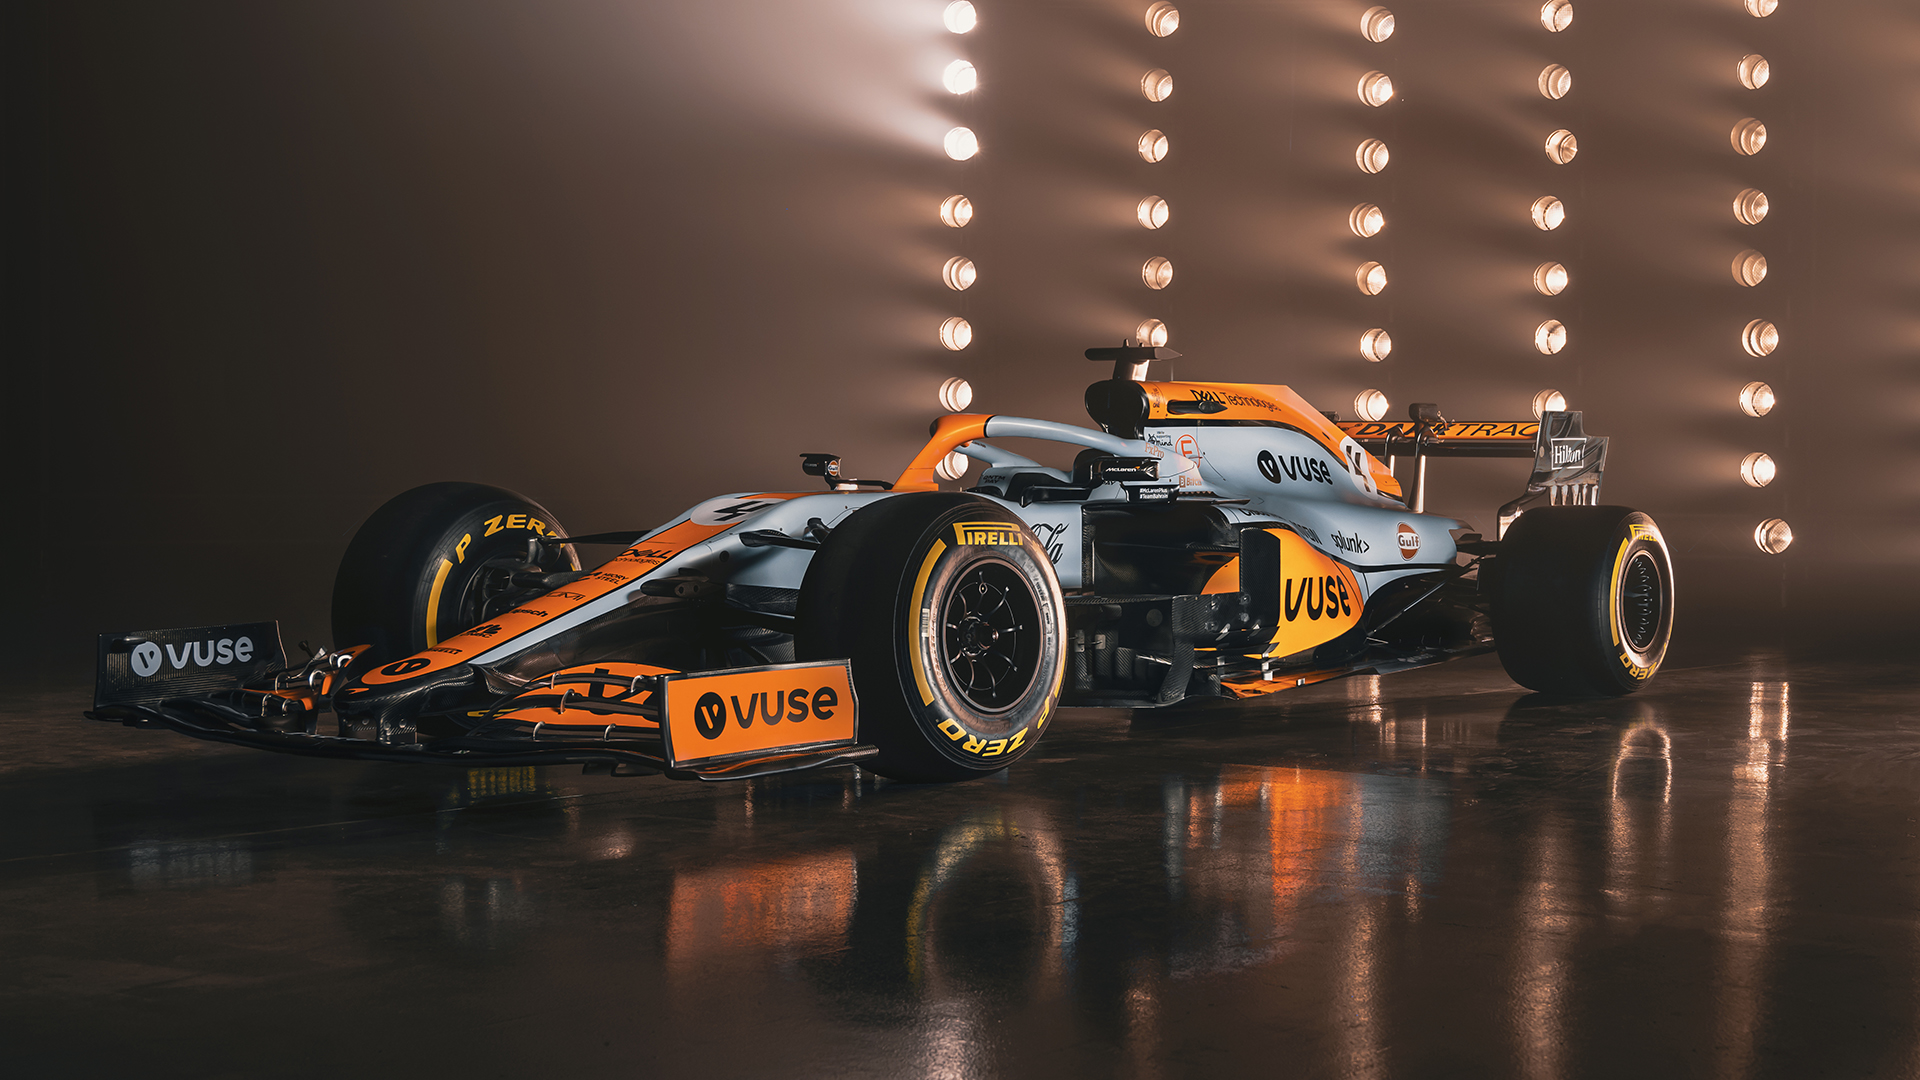
\includegraphics[height = 200pt]{pictures/artwojciech.png}
    \caption{Bolid Formuły 1(moje zdjęcie profilowe)}
\end{figure}

\newpage

\subsection{Tabela}
\label{tab: ściganie}

\begin{table}[h!]
\centering
\begin{tabular}{|l|l|}
\hline
\multicolumn{1}{|c|}{\textbf{Opony}} & \multicolumn{1}{c|}{\textbf{Trwałość}} \\ \hline
Miękkie                     & Słaba                         \\ \hline
Średnie                     & Średnia                       \\ \hline
Twarde                      & Duża                          \\ \hline
\end{tabular}
\end{table}


\subsection{Lista numerowana}

\begin{enumerate}
    \item RedBull
    \item Williams
    \item McLaren
    \item Mercedes
\end{enumerate}

\subsection{Lista nienumerowana}

\begin{itemize}
    \item banan
    \item jabłko
    \item mandarynka
\end{itemize}

\subsection{Krótki tekst}

\textbf{Formuła 1} to emocjonujący sport ekstremalny. Zawodnicy ścigają się w niej w specjalnie przygotowanych bolidach(\ref{fig: bolid}), kosztujących miliony dolarów. Wyścigi odbywają się na terenie \underline{całego świata}.
Na każdy tor co weekend zjeżdżają setki tysięcy kibiców. 

Aby wygrać, zespół \textbf{Formuły 1} musi nie tylko dysponować najszybszym samochodem i świetnym kierowcą, ale także odpowiednio dobrać strategię. Niezwykle istotny jest odpowiedni dobór opon(\ref{tab: ściganie}). W tym roku na torze królował \emph{Redbull}. \emph{\textbf{\large Zdobyli oni zarówno mistrzostwo kierowców, jak i konstruktorów. \normalsize}}